\documentclass[xcolor=table,aspectratio=169]{beamer}
\usepackage{beamerthemesplit}
\usepackage{wrapfig}
\usetheme{SPbGU}
\usepackage{pdfpages}
\usepackage{amsmath}
\usepackage{cmap}
\usepackage[T2A]{fontenc}
\usepackage[utf8]{inputenc}
\usepackage[english]{babel}
\usepackage{indentfirst}
\usepackage{mathtools}
\usepackage{tikz}
\usepackage{multirow}
\usepackage[noend]{algpseudocode}
\usepackage{algorithm}
\usepackage{algorithmicx}
\usepackage{fancyvrb}

\usepackage{minted}

\usetikzlibrary{calc}
\usetikzlibrary{shapes,arrows}
\usetikzlibrary{arrows,automata}
\usetikzlibrary{positioning}

\usepackage{fontawesome}

\usetikzlibrary{shapes.callouts}

\usepackage{xparse}

%for [[ ]]
\usepackage{stmaryrd}


\tikzset{
    invisible/.style={opacity=0,text opacity=0},
    visible on/.style={alt=#1{}{invisible}},
    alt/.code args={<#1>#2#3}{%
      \alt<#1>{\pgfkeysalso{#2}}{\pgfkeysalso{#3}} % \pgfkeysalso doesn't change the path
    },
}

\NewDocumentCommand{\mycallout}{r<> O{opacity=0.8,text opacity=1} m m m}{%
\tikz[remember picture, overlay]\node[align=center, fill=cyan!20, text width=#5cm,
#2,visible on=<#1>, rounded corners,
draw,rectangle callout,anchor=pointer,callout relative pointer={(230:1cm)}]
at (#3) {#4};
}

%\newcommand{\tikzmark}[1]{\tikz[overlay,remember picture,baseline=-0.5ex] \node (#1) {};}



\usepackage{tabularx}
\newcolumntype{Y}{>{\raggedleft\arraybackslash}X}

\renewcommand{\thealgorithm}{}

\newtheorem{mytheorem}{Theorem}
\renewcommand{\thealgorithm}{}

\newcommand{\tikzmark}[1]{\tikz[overlay,remember picture] \node (#1) {};}
\def\Put(#1,#2)#3{\leavevmode\makebox(0,0){\put(#1,#2){#3}}}

\newcommand{\ltz}{$< 1$}


\tikzset{
    state/.style={
           rectangle,
           rounded corners,
           draw=black, very thick,
           minimum height=2em,
           inner sep=2pt,
           text centered,
           },
}

\makeatletter
\AtBeginEnvironment{minted}{\dontdofcolorbox}
\def\dontdofcolorbox{\renewcommand\fcolorbox[4][]{##4}}
\makeatother

\beamertemplatenavigationsymbolsempty

\title[Магистерский грант 2021--2023]{Кандидаты на магистерский грант 2021--2023}
\institute[JB Research, SPbSU]{
JetBrains Research, Programming Languages and Tools Lab  \\
Saint Petersburg State University
}


\author[Семён Григорьев]{Семён Григорьев}

\date{31 мая 2021г.}

\begin{document}

{
\begin{frame}[fragile]
  \begin{tabular}{p{2.0cm} p{10.5cm} p{1cm}}
   \begin{center}
      
\includegraphics[height=1.5cm]{pictures/jetbrainsResearch.pdf}
    \end{center}
    &
    \begin{center}
      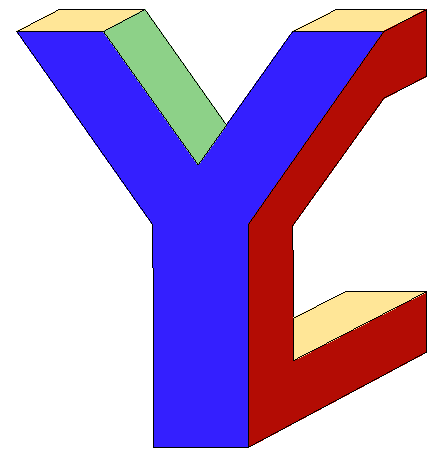
\includegraphics[height=1.5cm]{pictures/YC_logo.pdf}
    \end{center}
    &
    \begin{center}
      
\includegraphics[height=1.5cm]{pictures/SPbGU_Logo.png}
    \end{center}
  \end{tabular}
  \titlepage
\end{frame}
}

\begin{frame}[fragile] \frametitle{Орачев Егор Станиславович}
      \begin{minipage}[m]{0.45\linewidth}
  \raisebox{-0.5\totalheight}{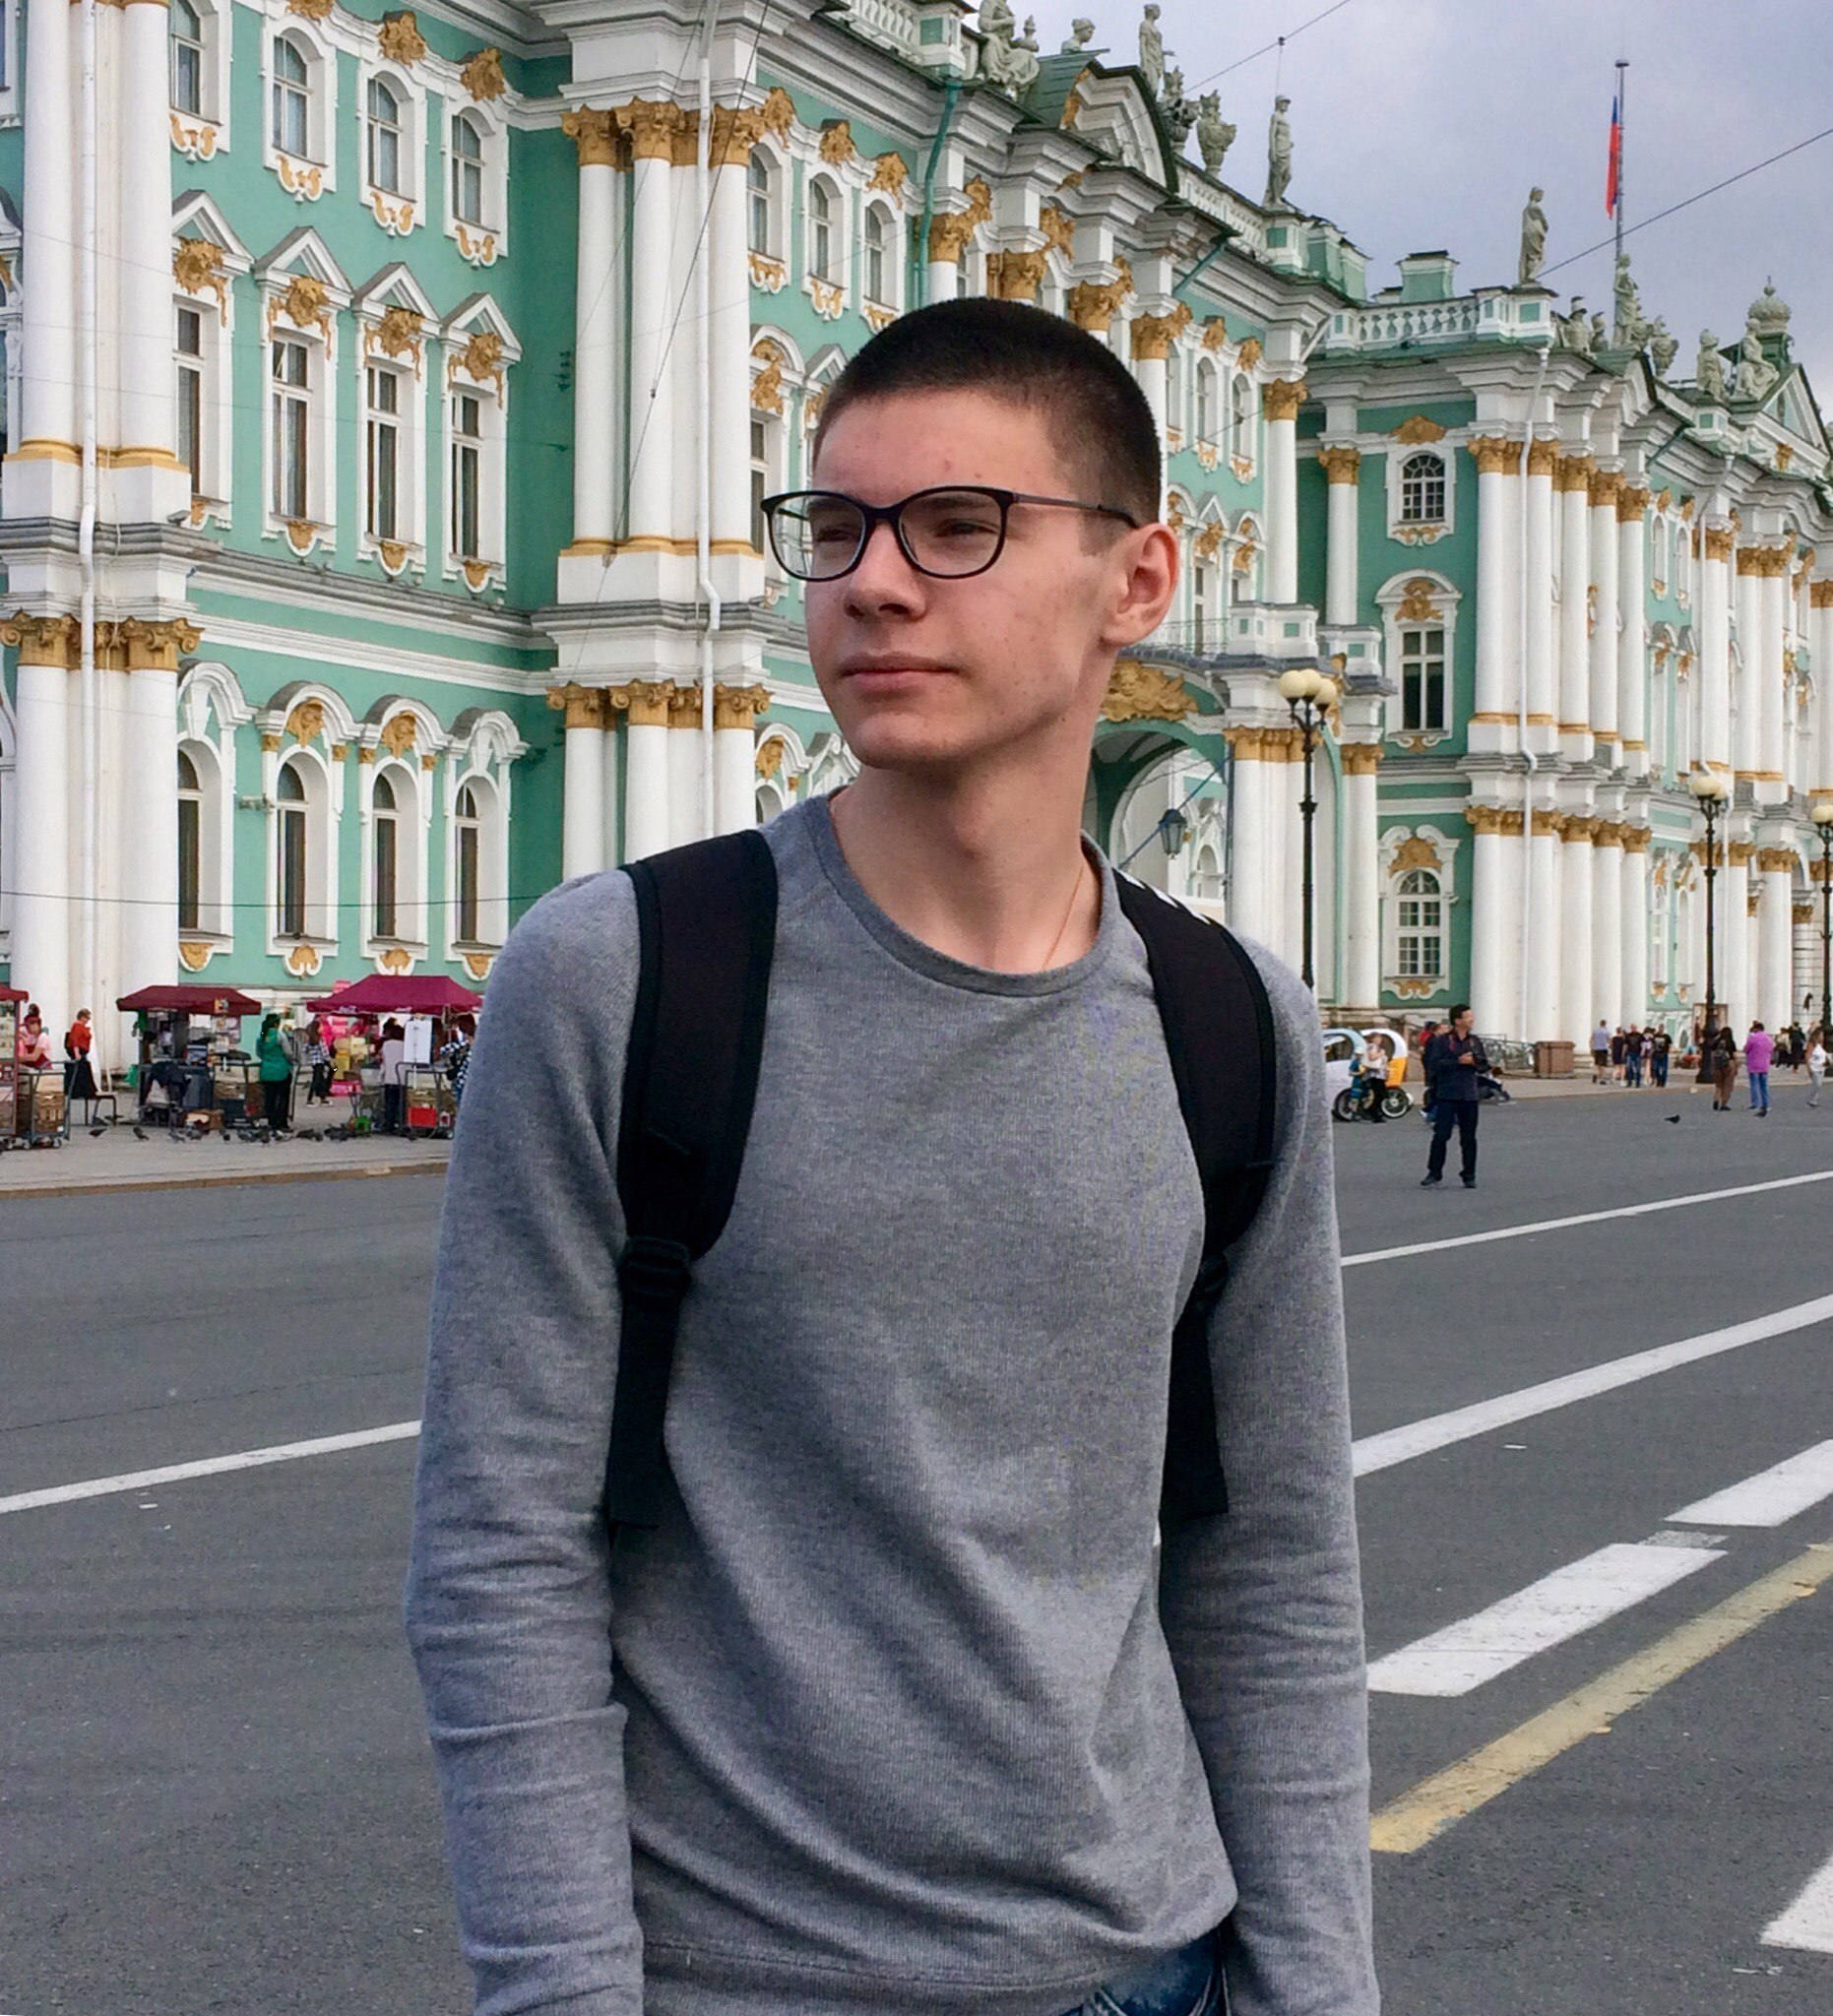
\includegraphics[width=\textwidth]{pictures/Orachev_ProfilePhoto.jpg}}
  \end{minipage}\hfill
  \begin{minipage}[m]{0.54\linewidth}
  Кандидат на магистерский грант

  \vfill

  \begin{itemize}
        \item Работает с нами с сентября 2019 года (3 курс, теория формальных языков)
        \item Закончит бакалавриат Мат-Мех факультета в июне 2021 года
        \item Тема ВКР бакалавра: ``Реализация алгоритма поиска путей в графовых базах данных через тензорное произведение на GPGPU''
        \item Получатель бакалаврского гранта
        \item Сфера интересов: высокопроизводительные вычисления на GPGPU, линейная алгебра, теория формальных языков и их приложения
  \end{itemize}
  \end{minipage}

\end{frame}


\begin{frame}[fragile] \frametitle{Исследовательская работа}
  
    \begin{itemize}
        \item Соавтор двух опубликованных работ
            \begin{itemize}
              \item ``Context-Free Path Querying by Kronecker Product''. \textbf{Egor Orachev}, Ilya Epelbaum, Rustam Azimov, Semyon Grigorev; 2020; Advances in Databases and Information Systems
              \item ``The Library of GPGPU-Powered Sparse Boolean Linear Algebra Operations''. \textbf{Egor Orachev}, Maria Karpenko, Artem Khoroshev, Semyon Grigorev; 2021; Workshop on Graphs, Architectures, Programming, and Learning (IPDPS).
            \end{itemize}

        \item И одного препринта: ``One Algorithm to Evaluate Them All: Unified Linear Algebra Based Approach to Evaluate Both Regular and Context-Free Path Queries''. Ekaterina Shemetova, Rustam Azimov, \textbf{Egor Orachev}, Ilya Epelbaum, Semyon Grigorev; 2021
        \item Автор и основной разработчик проектов \href{https://github.com/JetBrains-Research/cuBool}{cubool}, \href{https://pypi.org/project/pycubool/}{pycubool}, \href{https://github.com/JetBrains-Research/spbla}{spbla}
    \end{itemize}
  \pause
  \vfill
  Планы: инкрементальный распределённый межпроцедурный статический анализ на основе КС достижимости
  \begin{itemize}
        \item Экспериментальное исследование наших решений и сравнение с аналогами
        \item Разработка и реализация инкрементального алгоритма КС достижимости на основе линейной алгебры
        \item Участие в сообществе GraphBLAS (реализация стандарта на GPGPU)
  \end{itemize}

\end{frame}


\begin{frame}[fragile] \frametitle{Истомина Александра Андреевна}
  \begin{minipage}[m]{0.45\linewidth}
  \raisebox{-0.1\totalheight}{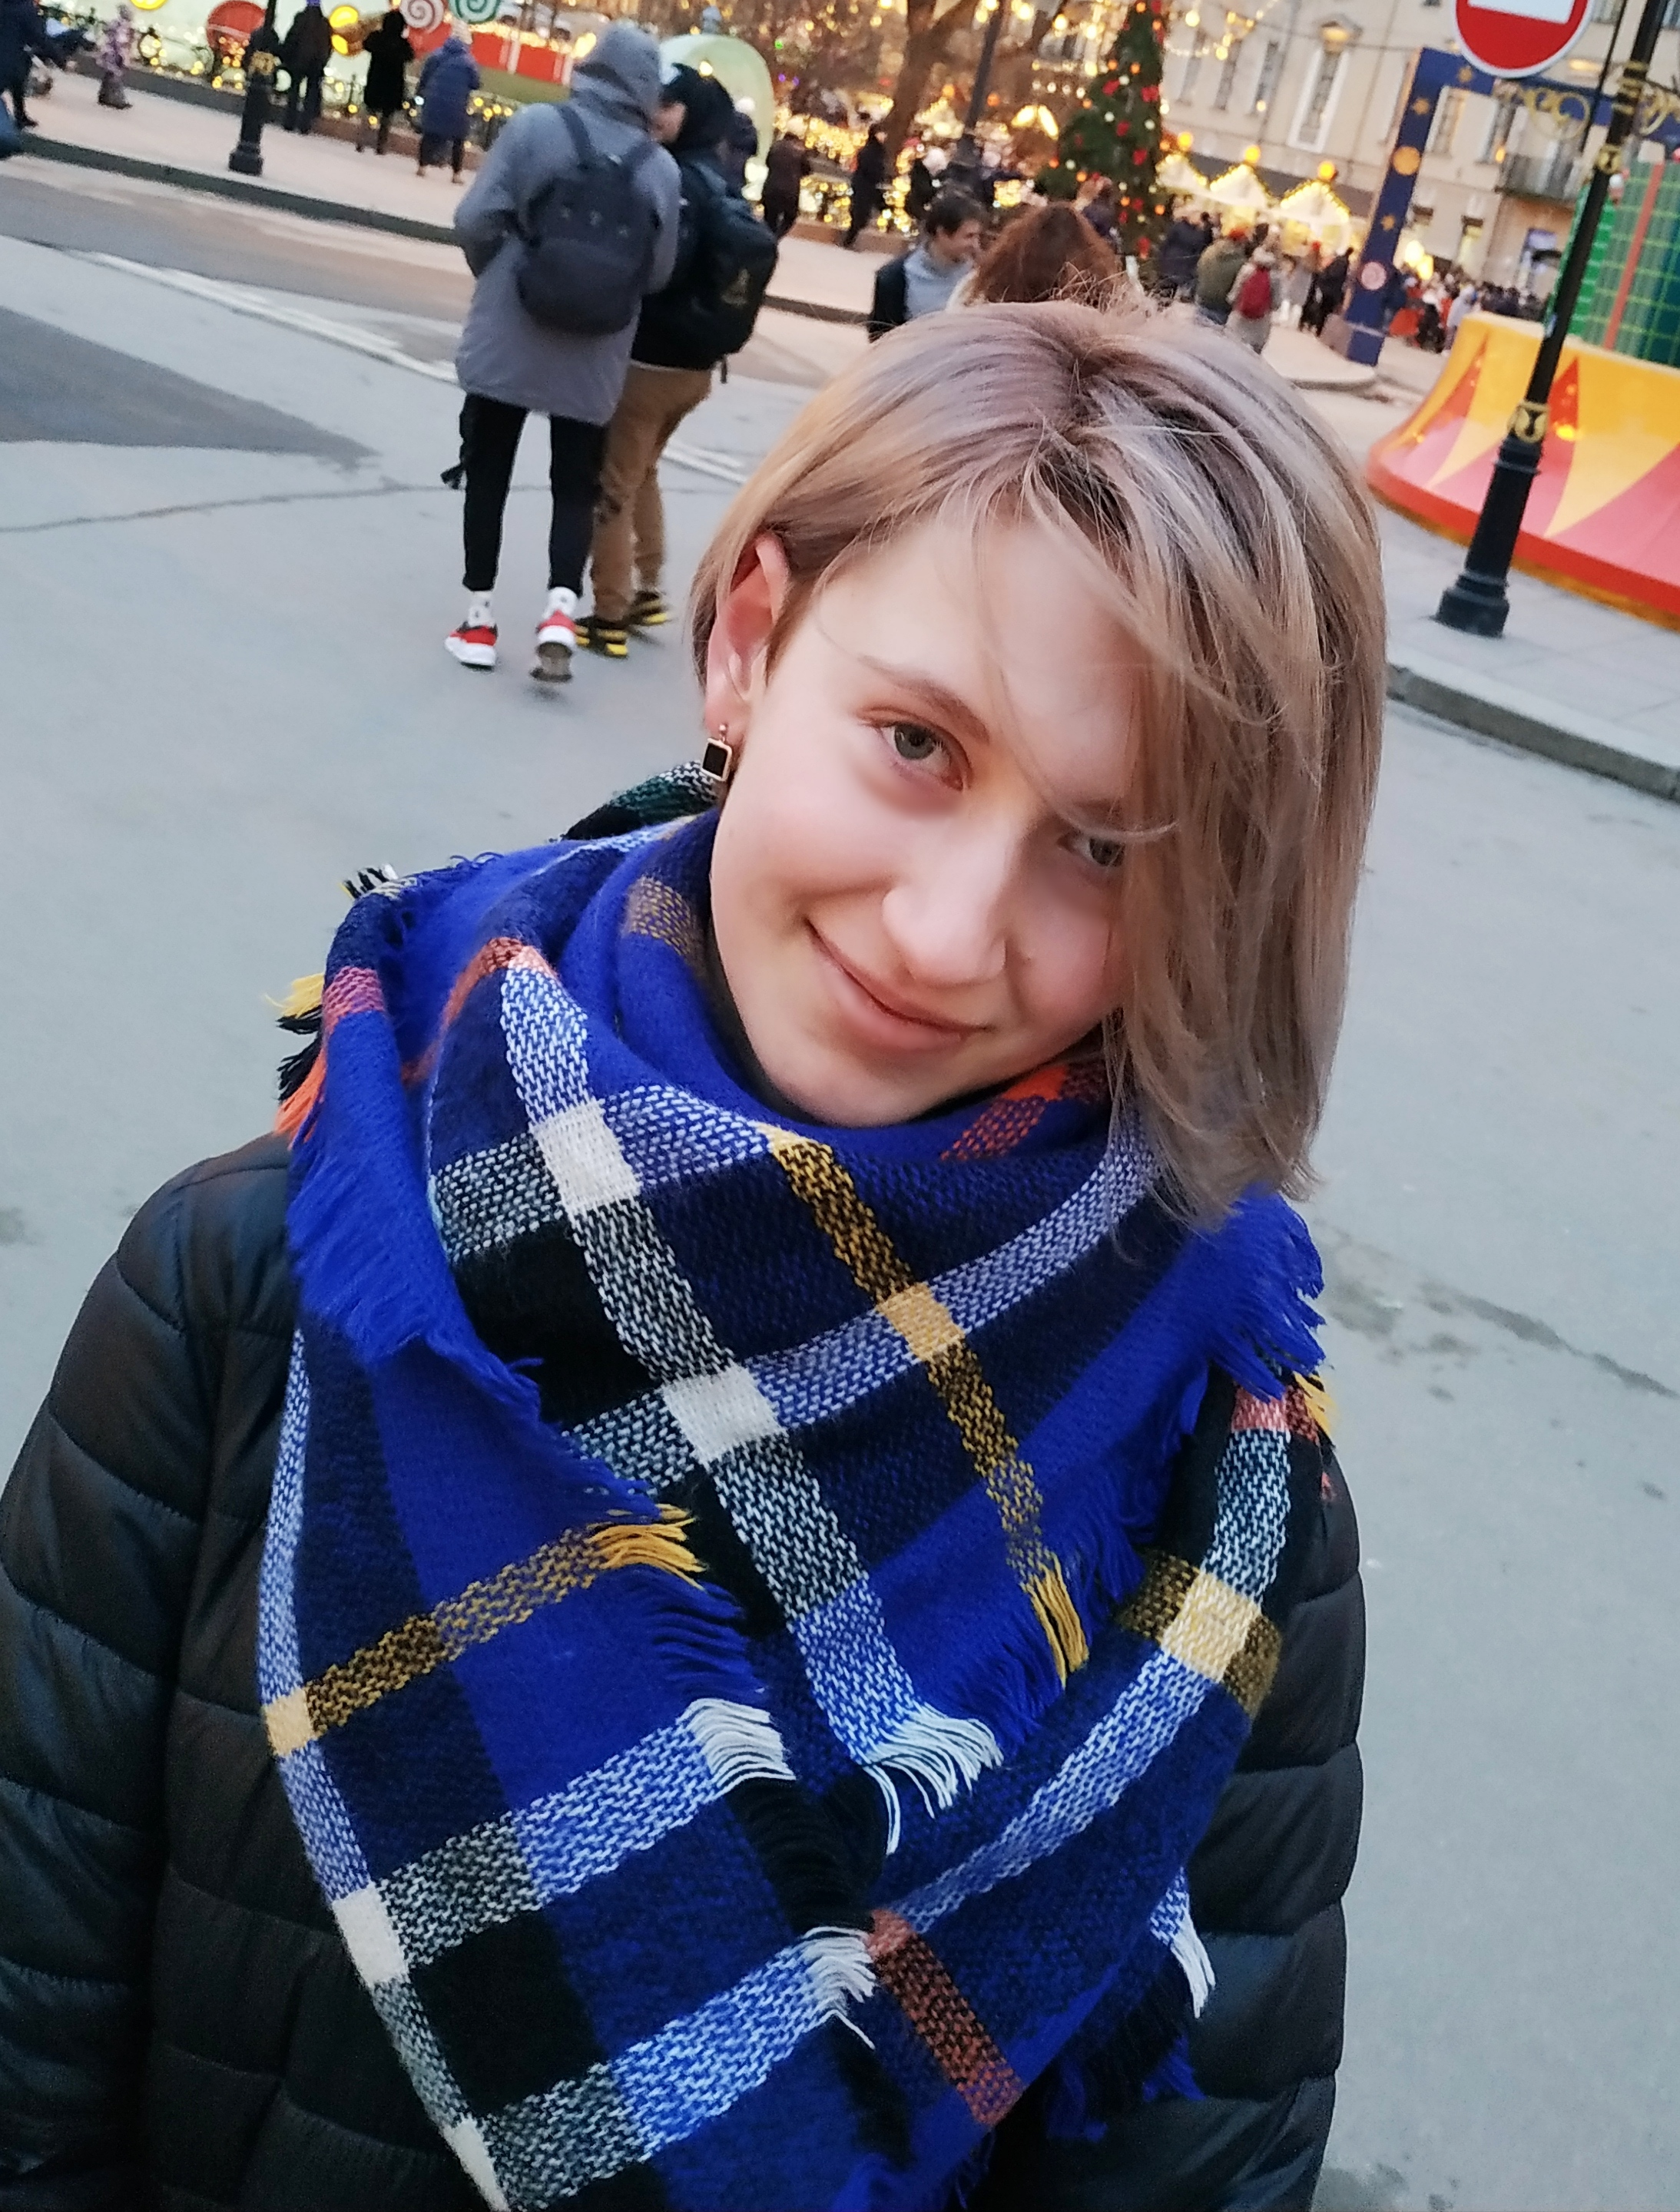
\includegraphics[width=\textwidth]{pictures/Istomina_ProfilePhoto.jpg}}
  \end{minipage}\hfill
  \begin{minipage}[m]{0.54\linewidth}
  \vspace{-1.6cm}
  Кандидат на магистерский грант
  \begin{itemize}
        \item Работает с нами с сентября 2020 года (семестровый проект CSC)
        \begin{itemize}
          \item Теоретическая сложность задчи достижимости с КС ограничениями в планарных графах
          \item Приглашена на стажировку
        \end{itemize}
        \item Окончила ГФМЛ 30 (золотая медаль)
        \item Закончит бакалавриат факультета МКН в июне 2021 года        
        \begin{itemize}
          \item Возможен красный диплом
        \end{itemize}
        \item Тема ВКР бакалавра: ``О морфинге изображений графов на плоскости и в пространстве''
        \begin{itemize}
          \item Научный руководитель: Арсеньева Елена Александровна
        \end{itemize}        
  
  \end{itemize}
  \end{minipage}

\end{frame}


\begin{frame}[fragile] \frametitle{Исследовательская работа}
  
    \begin{itemize}
        \item Сфера интересов: теория графов, геометрические алгоритмы, вероятностные алгоритмы
        \item Диплом 2 степени в олимпиаде ``Высшая лига'' по направлению ``Прикладная математика и информатика'' в 2021 году        
        \item Готовится статья на \href{https://algo.inf.uni-tuebingen.de/gd2021/}{Graph Drawing} (дедлайн 9 июня)
            \begin{itemize}
              \item По мотивам ВКР              
            \end{itemize}      
    \end{itemize}
  \pause
  \vfill
  Планы: исследование теоретических свойств задачи о достижимости с контекстно-свободными ограничениями
  \begin{itemize}
        \item Исследование теоретической сложности динамических вариантов задачи (меняется граф и/или граммтика)
        \item Исследование сводимости задачи КС достижимости в рамках мелкозернистой сложности, получение верхних и нижних оценок (совместно с Екатериной Шеметовой и Дмитрием Чистиковым)
  \end{itemize}

\end{frame}

\begin{frame}[fragile] \frametitle{Эпельбаум Илья Владимирович}
  \begin{minipage}[m]{0.45\linewidth}
  \raisebox{-0.1\totalheight}{\includegraphics[width=\textwidth]{pictures/Epelbaum_ProfilePhoto.png}}
  \end{minipage}\hfill
  \begin{minipage}[m]{0.54\linewidth}
  \vspace{-0.1cm}
  Кандидат на магистерский грант
  \begin{itemize}
        \item Работает с нами с сентября 2019 года (курсовая работа)
        \begin{itemize}
          \item ``Поиск путей в графовых базах данных через тензорное произведение''          
        \end{itemize}        
        \item Закончит бакалавриат Мат-Мех факультета в июне 2021 года                
        \item Тема ВКР бакалавра: ``Оптимизация алгоритма поиска путей сконтекстно-свободными ограничениями, основанногона произведении Кронекера''
        \item Получатель стипендии  
  \end{itemize}
  \end{minipage}

\end{frame}


\begin{frame}[fragile] \frametitle{Исследовательская работа}
  
    \begin{itemize}
        \item Сфера интересов: алгоритмы на графах, теория формальных языков и её приложения, линейная алгебра
        \item Соавтор двух опубликованных работ
            \begin{itemize}
              \item ``Context-Free Path Querying by Kronecker Product''. Egor Orachev, \textbf{Ilya Epelbaum}, Rustam Azimov, Semyon Grigorev; 2020; Advances in Databases and Information Systems
              \item ``Context-Free Path Querying with All-Path Semantics by Matrix Multiplication''. Rustam Azimov, \textbf{Ilya Epelbaum}, Semyon Grigorev; 2021; GRADES-NDA (SIGMOD).
            \end{itemize}

        \item И одного препринта: ``One Algorithm to Evaluate Them All: Unified Linear Algebra Based Approach to Evaluate Both Regular and Context-Free Path Queries''. Ekaterina Shemetova, Rustam Azimov, Egor Orachev, \textbf{Ilya Epelbaum}, Semyon Grigorev; 2021
        \item Основной разработчик проекта \href{https://github.com/JetBrains-Research/CFPQ_PyAlgo}{CFPQ\_PyAlgo}
    \end{itemize}
  \pause
  \vfill
  Планы: поиск путей с ограничениями в терминах многокомпонентных КС грамматик
  \begin{itemize}
        \item Разработка алгоритма на основе линейной алгебры
        \item Исследование теоретических свойст разработанного алгоритма
        \item Экспериментальное ислледование разработанного алгоритма и сравнение с аналогами (статический анализ кода)
  \end{itemize}

\end{frame}


\end{document}
